\chapter{Introduction}


\vspace{2mm}

\section{Motivation}
\textbf{Author: Sztavinovszki}

In almost every robotics application nowadays you need some kind of communication. Wether it is a robot communicating
its data to a home-base, or two robots sharing data with one another. Over the past years communication has drastically
improved with new protocols and technology, such as Bluetooth Low energy. On the other hand there are still people, that
don't use any of the communication technologies described before, because most of the established frameworks are seem to
complex or have too many requirements regarding performance.

\section{Goal}
\textbf{Author: Sztavinovszki}

This diploma thesis will take explore how to write a real-time communication framework using new technologies, such as BLE with TCP
and UDP.

At the end of the project the framework should be useable for sending data between two KIPR Wombat-Controllers. It should be capable
to send well structured data, e.g. a JSON-file, as well as streaming data, e.g. a series of pictures, between the robots. All sent data should have the
option to be compressed with different compression formats ranging from lossless to lossy formats. When using protocols, that don't make guarantees about
the completeness of the received data RECT will not provide extra safeguards to make sure all sent data is also received.
RECT should be able to provide a stable and fast connection at reasonable distances for the selected protocol (e.g. circa 30 meters of line-of-sight, for BLE).
RECT should provide libraries for the languages Python and C++ that hide the complexity of communication and provide nice abstractions simplifying its use.
For this to be made possible the following requirements have to be met:
\begin{Things to be done}
\item A Rust library for communicating via TCP, BLE and UDP has to be written.
\item A Rust gRPC service using the communication library has to be implemented.
\end{Things to be done}

\section{History}

\section{Project Management}
\textbf{Author: Sztavinovszki}
For the management of RECT Kanban was chosen, because of its low overhead and flexibility. Trello was chosen as the platform on which to use Kanban on, because of its simple setup and excellent features.

The project was hosted on \href{https://gitlab.htlwrn.ac.at/Sztavinovszki.Jeremy/RECT}{the schools gitlab server}, which also contained submodules hosted on \href{https://github.com/F-WuTS/}{F-WuTS} and on \href{https://github.com/if-loop69420}{Jeremy Sztavinovszki's personal github account}.

\section{Outline}
%\section{Section}
%More text. \lipsum[1] See Figure~\ref{pic:example}.

%\begin{figure}[h]
%	\centering
%	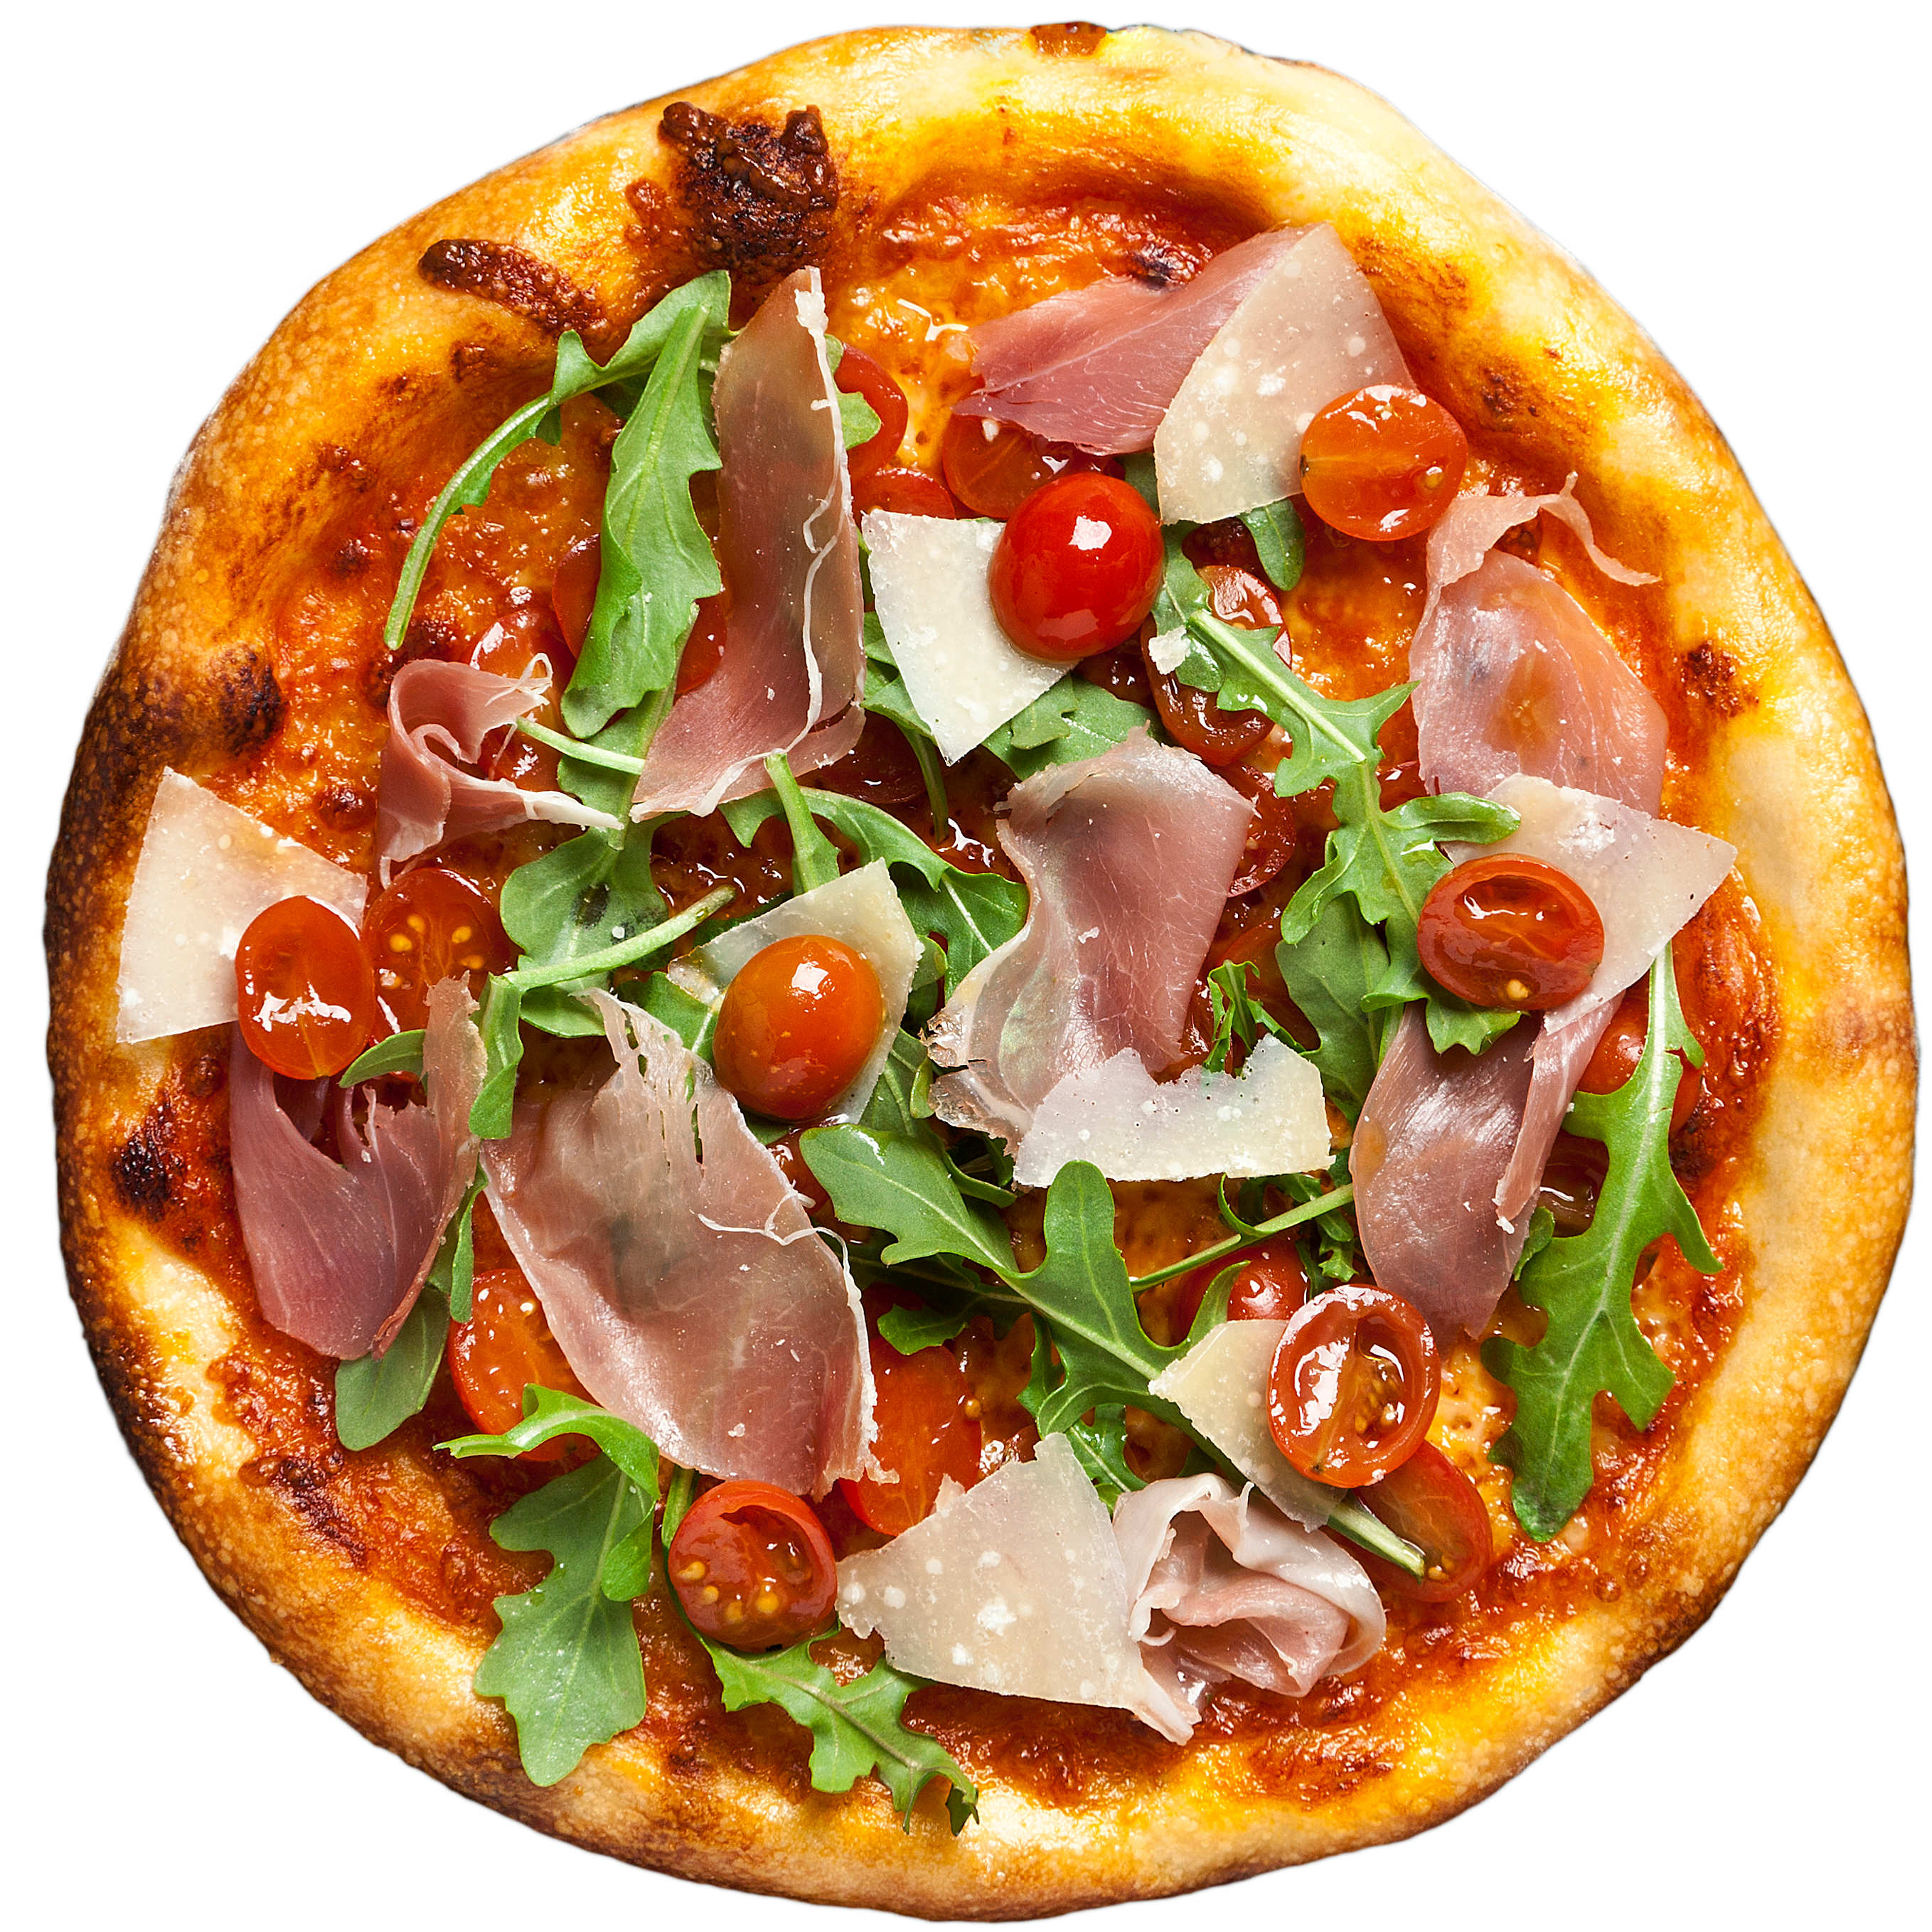
\includegraphics[width=2.5in]{img/example.png}
%	\caption{Picture description.}
%	\label{pic:example}
%\end{figure}

%\subsection{Subsection}
%\lipsum[1]

%\subsection{Subsection}
%\lipsum[1] See Table~\ref{tab:example}.

%\begin{center}
%	\begin{tabular}{| l | l | l |}
%		\hline
%		\bfseries Header 1 & \bfseries Header 2 & \bfseries Header 2 \\
%		\hline
%		Text & text & text \\
%		\hline
%		Text & text & text  \\
%		\hline
%		Text & text & text  \\
%		\hline
%	\end{tabular}
%	\label{tab:example}
%\end{center}

%\lipsum[1] Some references can be found at \footcite{robo4you} or at \footcite{Hope_Learning_TensorFlow}.
%

\filbreak
